\documentclass[tikz]{standalone}

\usepackage{fontspec}
\setmainfont[Ligatures=TeX, Mapping=tex-text]{Lato}
\usepackage{tikz}
\usepackage{xfp}

\begin{document}
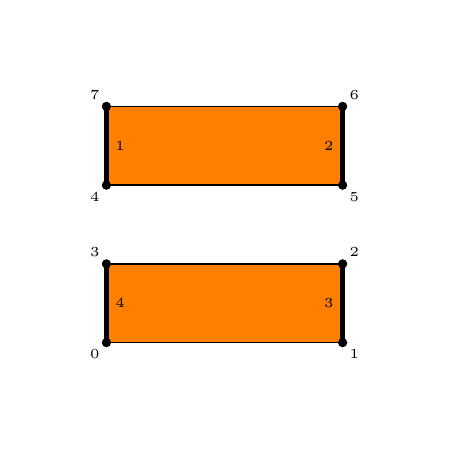
\begin{tikzpicture}

\def\width{5}
\def\height{5}
\def\ox{\fpeval{\width /2}}
\def\oy{\fpeval{\height /2}}

\tiny
\path [use as bounding box] (0,0) rectangle (\width,\height);

% SHAPE
\filldraw [line width=0.5pt, fill=orange] (\ox,\oy) ++(0,1)
	+(-1.5,-0.5) node[draw, fill=black, circle, inner sep=1pt] {} node[below left] {4} --
	+(1.5,-0.5) node[draw, fill=black, circle, inner sep=1pt] {} node[below right] {5} --
	+(1.5,0.5) node[draw, fill=black, circle, inner sep=1pt] {} node[above right] {6} --
	+(-1.5,0.5) node[draw, fill=black, circle, inner sep=1pt] {} node[above left] {7} --
	cycle;
\filldraw [line width=0.5pt, fill=orange] (\ox,\oy) ++(0,-1)
	+(-1.5,-0.5) node[draw, fill=black, circle, inner sep=1pt] {} node[below left] {0} --
	+(1.5,-0.5) node[draw, fill=black, circle, inner sep=1pt] {} node[below right] {1} --
	+(1.5,0.5) node[draw, fill=black, circle, inner sep=1pt] {} node[above right] {2} --
	+(-1.5,0.5) node[draw, fill=black, circle, inner sep=1pt] {} node[above left] {3} --
	cycle;

% PORTS
\draw [line width=2pt] (\ox,\oy) ++(-1.5,1) node[right] {1} +(0,-0.5) -- +(0,0.5);
\draw [line width=2pt] (\ox,\oy) ++(1.5,1) node[left] {2} +(0,-0.5) -- +(0,0.5);
\draw [line width=2pt] (\ox,\oy) ++(1.5,-1) node[left] {3} +(0,-0.5) -- +(0,0.5);
\draw [line width=2pt] (\ox,\oy) ++(-1.5,-1) node[right] {4} +(0,-0.5) -- +(0,0.5);

\end{tikzpicture}
\end{document}
